% !TeX root = ..\main.tex
\npchapter{Performanceanalyse}  \label{performanceAnalysis}
In diesem Kapitel wird die Performance von Bun detailliert betrachtet und mit Node.js verglichen. Hierbei liegt der Fokus darauf, die Leitfrage ``Welche konkreten Leistungsverbesserungen können in Bun 1.0 im Vergleich zu Node.js festgestellt werden, und wie lassen sie sich quantifizieren?'' zu beantworten. Zuerst wird die Vorgehensweise bei den Tests vorgestellt. Anschließend wird der verwendete Versuchsaufbau und die Beispielimplementierungen präsentiert. Darauffolgend werden die Ergebnisse der Tests analysiert.


\section{Vorgehensweise} \label{sec:performance-approach}
Als Metriken werden die durchschnittliche Latenz, die Anzahl an HTTP-Anfragen pro Sekunde, der Anteil an erfolgreichen HTTP-Anfragen, die CPU-Auslastung un der maximal genutzte Arbeitsspeicher während der Ausführungszeit (siehe Kapitel \ref{sec:foundations-Performance})\todo{Verifizieren, dass die Metriken dort inkludiert sind}. Um diese Metriken zu ermitteln, werden verschiedene Szenarien inklusive unterschiedlicher Implementierungen verwendet (siehe Kapitel \ref{sec:performance-implementations}). Die unterschiedlichen Implementierungen sind auf variierende APIs \todo{Abkürzung einführen, falls in Theorie nicht geschehen} der Laufzeitumgebungen zurückzuführen. Diese müssen verwendet werden, damit die Leistung der Laufzeitumgebungen und nicht die Performance des Quellcodes geprüft wird.\\

\noindent
Zuerst wird die grundlegende Performance von HTTP-Server beider Laufzeitumgebungen gemessen (siehe Kapitel \ref{subsec:httpServer}). Es greifen 500 gleichzeitige Benutzer auf den Server für 30 Sekunden lang zu und erhalten einen String als Antwort zurück. Dieses Szenario veranschaulicht die grundlegende Netzwerkgeschwindigkeit beider Laufzeitumgebungen. Als zweites Szenario wird ein Datei-Server verwendet, der jedem Aufrufer ein Bild zurückgibt (siehe Kapitel \ref{subsec:fileServer}). Diese Aufgabe wird für 50, 250, 500 und 1000 gleichzeitige Nutzer für eine Dauer von 30 Sekunden gemessen. Die Last wird variiert, um die Server näher an ihre Grenzen zu bringen. Der letzte Testfall berechnet die Fibonacci-Folge für die Zahl 45, damit die Leistung beider Laufzeitumgebungen bei rechenintensiven Aufgaben evaluiert wird (siehe Kapitel \ref{subsec:fibonacci}).

\noindent
Um die Performance korrekt zu bestimmen, müssen die richtigen Tools verwendet werden. In dieser Arbeit werden die Folgenden genutzt:

\begin{itemize}
	\item Bombardier,
	\item GNU Time.
\end{itemize}

\noindent
Bombardier generiert die HTTP-Anfragen an die Server im ersten und zweiten Testszenario. Im Tool kann die Dauer der Lasttests oder auch die Anzahl an zu versendeten Anfragen konfiguriert werden. Zusätzlich kann per Parameter bestimmt werden, wie viele gleichzeitige Benutzer simuliert werden. Nach dem Test gibt das Tool für die Anzahl an Anfragen pro Sekunde und für die Latenz die durchschnittlichen und maximalen Werte sowie die Standardabweichung aus. Zusätzlich kann der Anteil an erfolgreichen Anfragen bestimmt werden. Denn Bombardier gibt auch die Anzahl an Anfragen pro HTTP-Statuscode aus. Das Tool eignet sich aufgrund seinen detailreichen Aufgaben und seiner Performance. Es ist in Go geschrieben und verwendet das Paket ``fasthttp`` statt der nativen HTTP-Implementierung von Go und ist dadurch ausreichend performant. Damit die CPU-Auslastung und der maximal verwendete Arbeitsspeicher in den Ergebnissen berücksichtigt werden kann, wird GNU Time verwendet. GNU Time ist in Ubuntu bereits nativ verfügbar und eignet sich dadurch. Auf MacOS wird eine entsprechende Portierung dieses Tools verwendet, um vergleichbare Daten zu erheben. \newline
Um ein möglichst repräsentatives Ergebnis zu erhalten, wird jedes Testszenario für jede Laufzeitumgebung jeweils 5-mal ausgeführt. Aus den gesammelten Daten wird pro Eigenschaft der Durchschnitt gebildet. Dadurch fallen einzelne Ausreißer weniger ins Gewicht.

\noindent
Die vorgestellte Testkonfiguration ermöglicht die Quantifizierung der Performance-Metriken, um aus diesen Metriken fundierte Aussagen über die Performance beider Laufzeitumgebungen ableiten zu können und die 1. Forschungsfrage (siehe Kapitel \ref{sec:introduction-target}) zu beantworten.


\section{Versuchsaufbau} \label{sec:performance-testSetup}
Um eine konsistente und kontrollierte Umgebung für die Tests zu schaffen, werden diese auf spezifischer Hardware und Software durchgeführt. Das Ziel besteht darin, die Testergebnisse so reproduzierbar wie möglich zu gestalten. Des Weiteren wird dadurch eine Vergleichbarkeit zwischen Bun und Node.js gewährleistet, was die Quantifizierung der verwendeten Metriken ermöglicht.

\begin{table}[h]
	\centering
	\begin{tabular}{|p{3cm}|p{3cm}|p{3cm}|p{3cm}|}
		\hline
		Name & Desktop-PC & MacBook Pro \\
		\hline
		Prozessor & AMD Ryzen 7 2700 @ 3,6 GHz & Apple M1 Pro \\
		\hline
		Arbeitsspeicher & 32 GB DDR4-3200 & 16 GB LPDDR5-6400 \\
		\hline
		Betriebssystem & Ubuntu 23.10 & macOS 14 Sonoma \\
		\hline
	\end{tabular}
	\caption{Hardware für die Performanceanalyse}
	\label{table:hardware}
\end{table}

\noindent
Die Tests werden auf verschiedenen Geräten mit unterschiedlichen Betriebssystemen durchgeführt, wie in Tabelle \ref{table:hardware} dargestellt. Dies dient der Verifikation, ob etwaige Performance-Verbesserungen auf eine spezifische Systemumgebung zurückzuführen sind. Die native Implementierung von Bun für Windows ist experimentell und nicht vollständig für die Performance optimiert (siehe Kapitel \ref{sec:foundations-Bun}). Die experimentelle Lösung ist nicht für die Öffentlichkeit zugänglich \cite{Verhelst.2023}. Daher kann die Funktionsweise von Bun unter Windows nicht getestet werden.

\noindent
Um die tatsächlichen Tests auszuführen, werden die folgenden Versionen der betrachteten Frameworks verwendet:
\begin{itemize}
	\item Bun Version 1.0.6 (Neuste Version)
	\item Node.js Version 18.18.2 (LTS)
	\item Node.js Version 21.0.0 (Neuste)
\end{itemize}
\todo{Vermwerk, zu welchem Datum es sich um die aktuellsten Versionen handelt}

\noindent
Die neuste Version von Bun wird für die Tests verwendet, da sie im Vergleich zur Version 1.0 bereits Fehlerkorrekturen enthält \cite{Sumner.2023}. Bei der Analyse von Node.js werden zwei Versionen einbezogen. Zum einen die Version mit Long Term Support (LTS), da Node.js diese Version für die meisten Benutzer aufgrund des langfristigen Supports empfiehlt \cite{OpenJSFoundation.o.J.}. Zum anderen die neuste Version von Node,js, da in Version 20 beispielsweise die neuste Version des URL-Parsers Ada eingeführt wurde, die signifikante Performance-Verbesserungen mit sich bringt \cite{OpenJSFoundation.2023}. Zusätzlich enthält Version 21 weitere kleine Verbesserungen hinsichtlich der Performance \cite{OpenJSFoundation.2023b}.


\section{Implementierungen} \label{sec:performance-implementations}
Im Folgenden werden die verwendeten Implementierungen für jedes Testszenario (siehe Kapitel \ref{sec:performance-approach}) vorgestellt.

\subsection{HTTP-Server} \label{subsec:httpServer}
Um die grundlegende Performance von Netzwerkanfragen zu bestimmen, werden die zwei einfache Programme verwendet. Abbildung  \ref{fig:httpServerBun} zeigt den Quellcode für Bun, Abbildung \ref{fig:httpServerNode} für Node.js.

\begin{lstlisting}[caption={HTTP-Server Bun},label={fig:httpServerBun}]
	Bun.serve({
		port: 3000,
		fetch(request) {
			return new Response("Hello from Bun!");
		},
	});
\end{lstlisting}

\begin{lstlisting}[caption={HTTP-Server Node.js},label={fig:httpServerNode}]
	import http from "node:http";
	
	http.createServer(function (request, response) {
		response.write('Hello from Node.js!')
		response.end();
	}).listen(3000);
\end{lstlisting}

\noindent
Um die Performance der ersten beiden Programme zu testen, werden mit Bombardier 500 gleichzeitige Benutzer für eine Dauer von 30 Sekunden simuliert. Der dafür notwendige Befehl wird in Abbildung \ref{fig:bombardierHttpServer} visualisiert.
\begin{lstlisting}[caption={Bombardier HTTP-Server},label={fig:bombardierHttpServer}]
	bombardier -c 500 -d 30s http://localhost:3000
\end{lstlisting}

\noindent
Die Server wurden mit der entsprechenden Laufzeitumgebung gestartet. Um die Auslastung der CPU und des RAMs zu bestimmen, wird GNU Time benutzt. Der dafür erforderliche Befehl wird in Abbildung \ref{fig:timeHTTPServerUbuntu} für Ubuntu und in Abbildung \ref{fig:timeHTTPServerMacOS} für MacOS dargestellt. In MacOS wurde ``gtime`` genutzt, das eine Portierung von ``time`` unter Linux ist.

\begin{lstlisting}[caption={Bombardier HTTP-Server},label={fig:timeHTTPServerUbuntu}]
	/usr/bin/time -f "Execution Time: %e\nMaximum Resident Set Size (RSS): %M\nPercent of CPU This Job Got: %P" bun httpServer.js
\end{lstlisting}

\begin{lstlisting}[caption={Bombardier HTTP-Server},label={fig:timeHTTPServerMacOS}]
	gtime -f "Execution Time: %e\nMaximum Resident Set Size (RSS): %M\nPercent of CPU This Job Got: %P" bun httpServer.js
\end{lstlisting}

\subsection{File-Server} \label{subsec:fileServer}
Eine häufige Aufgabe von Web-Servern ist es, Bilder für das Frontend zur Verfügung zu stellen \todo{Quelle?}. Daher wird dieses Szenario als Nächstes gemessen, um auch die Performance von Zugriffe auf das Dateisystem in den Vergleich einfließen zu lassen. \newline
Abbildung  \ref{fig:fileServerBun} zeigt die Implementation für Bun, Abbildung \ref{fig:fileServerNode} für Node.js.

\begin{lstlisting}[caption={File-Server Bun.js},label={fig:fileServerBun}]
	const basePath = "../data";
	
	Bun.serve({
		port: 3000,
		fetch(request) {
			const filePath = `${basePath}${new URL(request.url).pathname}`;
			
			try {
				return new Response(Bun.file(filePath));
			} catch (error) {
				return new Response("File not found", {
					status: 404
				});
			}
		},
	});
\end{lstlisting}

\begin{lstlisting}[caption={File-Server Node.js},label={fig:fileServerNode}]
	import { createReadStream } from "node:fs";
	import http from "node:http";
	
	const basePath = "../data";
	
	http.createServer((request, response) => {
		const filePath = `${basePath}${request.url}`;
		const readStream = createReadStream(filePath);
		
		readStream.on("open", () => {
			response.setHeader("content-type", "image/png");
			response.writeHead(200);
			
			readStream.pipe(response);
		});
		
		readStream.on("error", () => {
			response.writeHead(404, "Image not found");
			response.end();
		});
	}).listen(3000);
\end{lstlisting}

\noindent
Mit Hilfe von Bombardier rufen beide Server dasselbe Bild aus dem Dateisystem ab. Falls dieses nicht gefunden wird, geben beide eine entsprechende Fehlermeldung zurück. Dieses Testszenario wird jeweils mit 50, 250, 500 und 1000 gleichzeitigen Benutzern für eine Dauer von 30 Sekunden getestet (siehe Kapitel \ref{sec:performance-approach}). Abbildung  \ref{fig:bombardierFileServer} zeigt das resultierende Kommando für 50 gleichzeitige Nutzer. Die Befehle zum Messen der CPU- und RAM-Auslastung unterscheiden sich nicht im Vergleich zum HTTP-Server (siehe Kapitel \ref{subsec:httpServer}).

\begin{lstlisting}[caption={Bombardier File-Server},label={fig:bombardierFileServer}]
	bombardier -c 500 -d 30s http://localhost:3000/example.png
\end{lstlisting}

\subsection{Fibonacci} \label{subsec:fibonacci}
Als letztes Szenario wird die Fibonacci-Folge für die Zahl 45 berechnet, um die Leistung bei der Ausführung rechenintensiver Aufgaben zu bewerten. Hierfür nutzen beide Laufzeitumgebungen die in Abbildung \ref{fig:fibonacci} dargestellte Implementierung.

\begin{lstlisting}[caption={Berechnung der Fibonacci-Folge},label={fig:fibonacci}]
	const fibonacci = (number) => {
		if (number <= 0) {
			return 0;
		} else if (number <= 1) {
			return 1;
		} else if (number <= 2) {
			return 2;
		}
		
		return fibonacci(number-1) + fibonacci(number-2);
	};
	
	console.log(fibonacci(45));
\end{lstlisting}

\noindent
Das Programm wird mit beiden Laufzeitumgebungen und GNU Time zur Erhebung der notwendigen Metriken ausgeführt. Abbildung \ref{fig:timefibonacciUbuntu} stellt dies beispielsweise für Node.js unter Ubuntu dar. Auf MacOS muss ``/usr/bin/time`` durch ``gtime`` ersetzt werden.
\begin{lstlisting}[caption={Fibonacci Node.js},label={fig:timefibonacciUbuntu}]
	/usr/bin/time -f "Execution Time: %e\nMaximum Resident Set Size (RSS): %M\nPercent of CPU This Job Got: %P" node fibonacci.js
\end{lstlisting}



\section{Ergebnisse} \label{sec:performance-results}
Im Folgenden werden die Ergebnisse der Testszenarien vorgestellt. Im Anschluss folgt die Diskussion über mögliche Konsequenzen.\\


\begin{figure}[h]
	\centering
	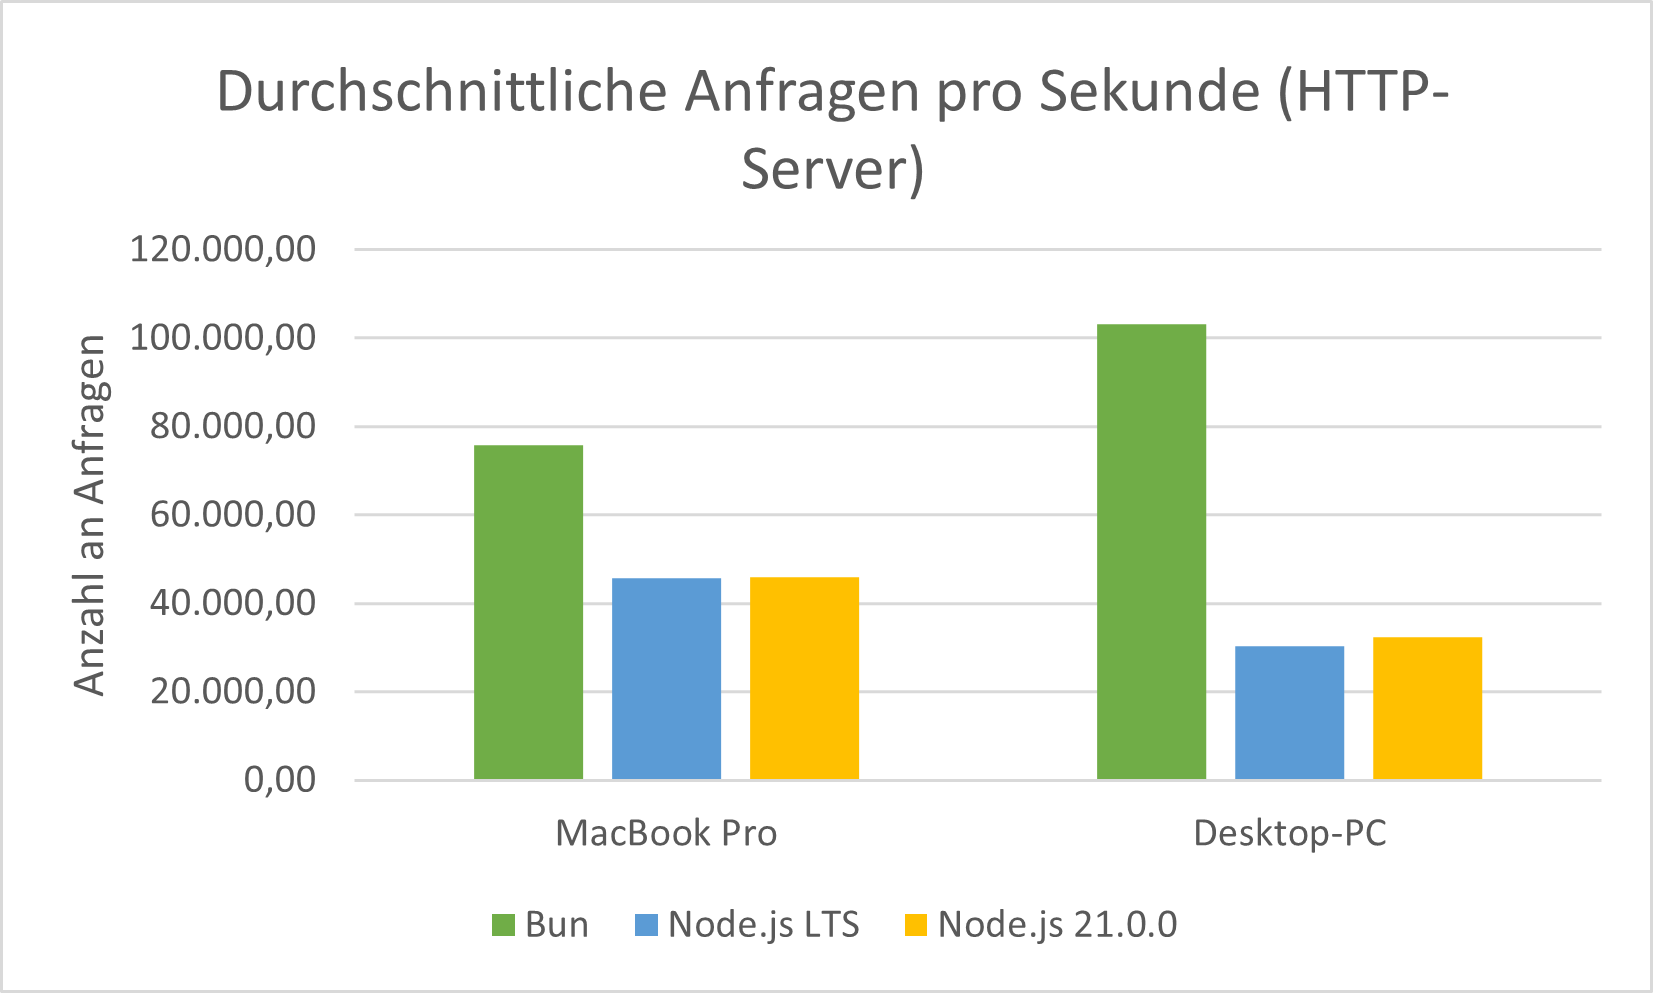
\includegraphics[width=\linewidth]{./images/httpServerAverageRequestsPerSecond.png}
	\caption{HTTP-Server - Durchschnittliche Anzahl an Anfragen pro Sekunde}
	\label{fig:httpServerAverageRequestsPerSecond}
\end{figure}


\noindent
Im ersten Testszenario wurde die grundlegende Leistung der HTTP-Server verglichen. Abbildung \ref{fig:httpServerAverageRequestsPerSecond} zeigt die durchschnittliche Anzahl an Anfragen pro Sekunde, die jede Laufzeitumgebung bei 500 Benutzern bewältigen konnte. Bun hat auf beiden Endgeräten deutlich besser abgeschnitten als die Node.js, unabhängig von dessen Version. Bun konnte auf dem Desktop-PC pro Sekunde ungefähr 103.000 Anfragen bewältigen, Node.js nur 30.000 (LTS) und 32.000 (Latest). Derselbe Sachverhalt macht sich auch in den Latenzzeiten bemerkbar. Bun hatte eine Latenz von 6,61ms auf dem MacBook Pro und 4,84ms auf dem Desktop-PC \todo{Diagramm im Anhang hinzufügen}. Im Vergleich musste ein Benutzer bei Node.js ungefähr 10ms auf dem MacBook Pro und ca. 16ms auf dem Desktop-PC auf eine Antwort warten.\newline
Dieser signifikante Unterschied zeigt, dass Bun Potential bietet auch in realen Szenarien deutlich schneller zu sein als Node.js. Der erste Test zeigt, dass die Verwendung der JavaScriptCore Engine und Zig als Programmiersprache Vorteile zu bieten scheint. In der Produktionsumgebung können so mehrere gleichzeitige Nutzer ohne Performanceverluste bedient werden.\\

\begin{figure}[h]
	\centering
	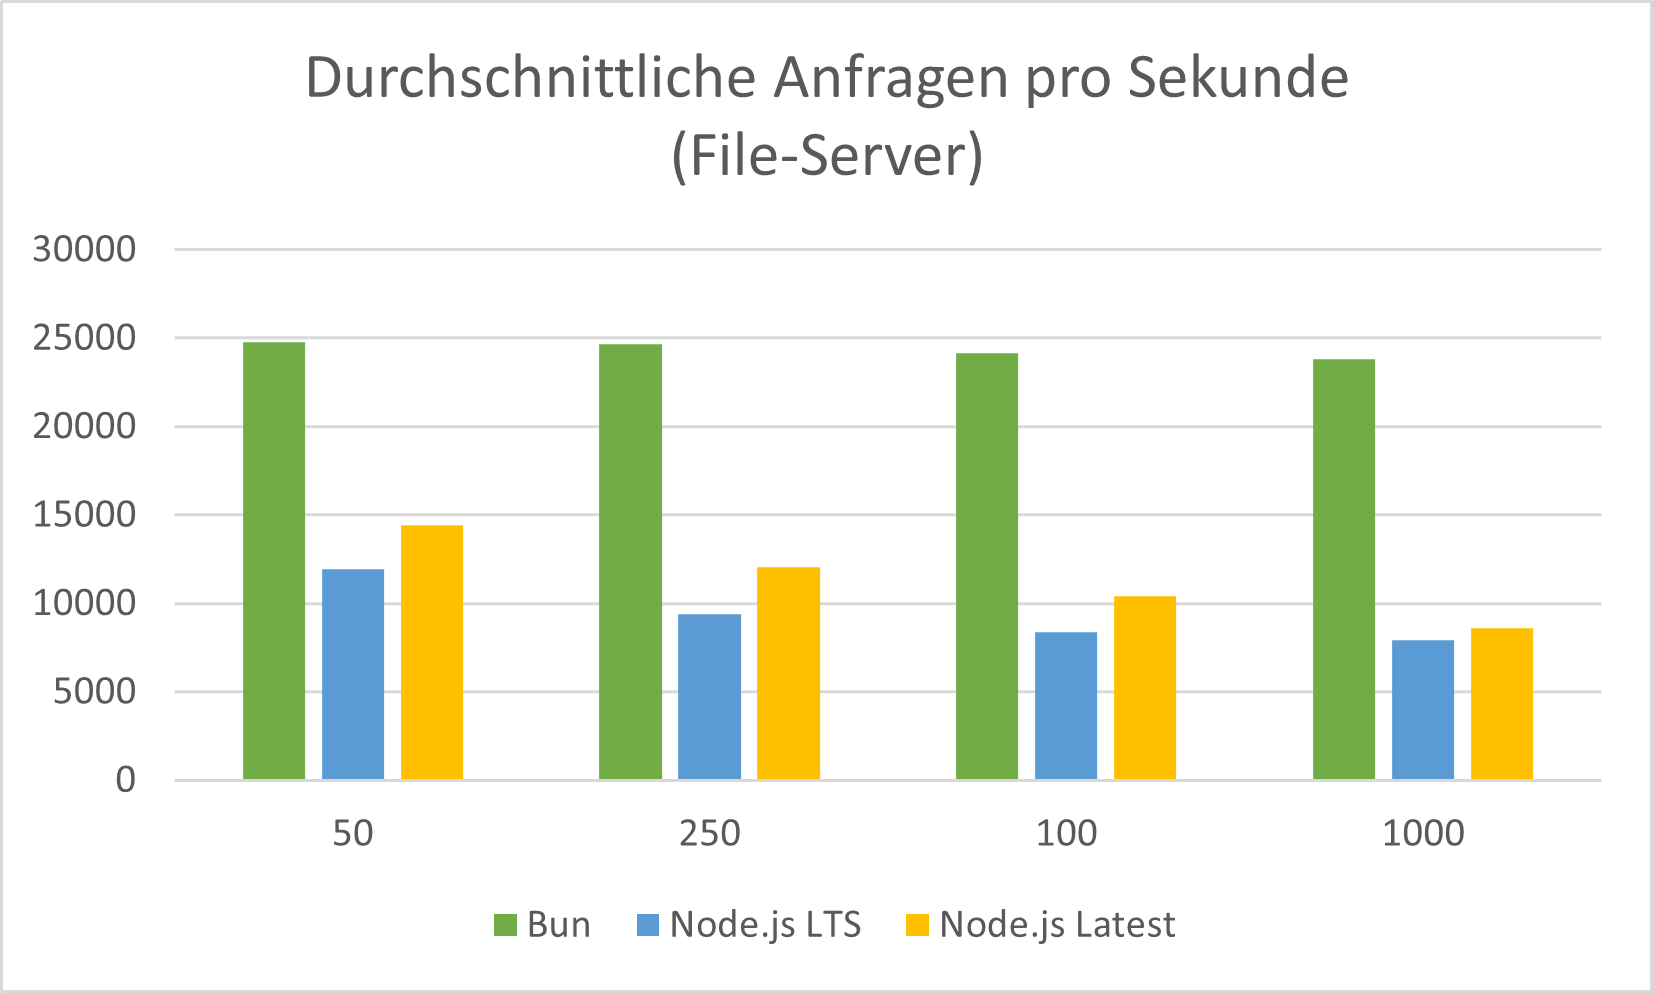
\includegraphics[width=\linewidth]{./images/fileServerAverageLatencyDesktop.png}
	\caption{File-Server - Durchschnittliche Latenz}
	\label{fig:fileServerAverageLatency}
\end{figure}

\noindent
Das zweite Testszenario analysiert, inwiefern die Potentiale aus dem ersten Test in einem realen Anwendungsfall umgesetzt werden. Um die Diagramme übersichtlich zu halten, konzentriert sich die Darstellung auf den Desktop-PC. Denn die Unterschiede und Trends sind auf beiden Geräten ähnlich. Abbildung \ref{fig:fileServerAverageLatency} zeigt die durchschnittlichen Latenzzeiten beim Zugriff auf ein Bilddatei, die an den Aufrufer zurückgegeben wird. Bun schneidet deutlich besser ab als Node.js. Dies ist über alle 4 Vergleichsszenarien zu beobachten. Bei 50 gleichzeitigen Benutzern hat Bun eine Latenzzeit von 2ms, währned Node.js eine Latenz von 4,2ms (LTS) bzw. 3,5ms (Latest) aufweist. Der Unterschied zwischen Bun und Node.js wächst mit der Anzahl an gleichzeitigen Benutzern an. Bei 250 Nutzern beläuft sich Buns Latenz auf ca. 10ms, der beste Wert von Node.js liegt bei ca. 21ms (Latest). Bei 1000 gleichzeitigen Nutzern benötigt Node.js im Durchschnitt für ca. 116ms (Latest) für die Antwort ein den Benutzer. Bun schafft es dagegen in ca. 42ms. Die Unterschiede betragen teilweise mehr als 50\%. Dies führt zu drastischen Unterschieden bei der Ladezeit von Webseiten, wenn Bilder teilweise mehr als 50\% schneller geladen werden können. Dadurch, dass Bun die Anfragen selbst deutlich schneller beantwortet, bewältigt Bun gleichzeitig deutlich mehr Anfragen pro Sekunde. Dies ist unabhängig von der Anzahl an gleichzeitigen Benutzern. Auf dem Desktop-PC schaffen es alle Laufzeitumgebungen alle gesendeten Anfragen erfolgreich zu beantworten. Auf dem MacBook Pro beantwortet Bun bei 50, 250 und 500 gleichzeitigen Anwendern alle Anfragen erfolgreich. Bei 1000 Nutzern sinkt der Wert auf 99,96\%. Die LTS-Version von Node.js liefert auch erst bei 1000 gleichzeitigen Benutzern fehlerhafte Antworten zurück. Der Anteil erfolgreicher Anfragen beläuft sich auf 99,92\%. Erst bei der neusten Version von Node.js treten Unterschiede zu Bun und Node.js LTS auf. Diese neuste Version beantwortet ab 250 gleichzeitigen Nutzern nicht mehr alle Anfragen erfolgreich. Bei 1000 Nutzern sinkt der Wert auf 99,54\%. Die absolute Anzahl an Anfragen, die mit einem Fehler beantwortet wurden, ist sehr niedrig. Dennoch ist es sehr auffällig, dass die neuste Version von Node.js hier deutlich größere Defizite aufweist. Möglicherweise ist hier auch noch ein Fehler im neusten Release enthalten.\\

\begin{figure}[h]
	\centering
	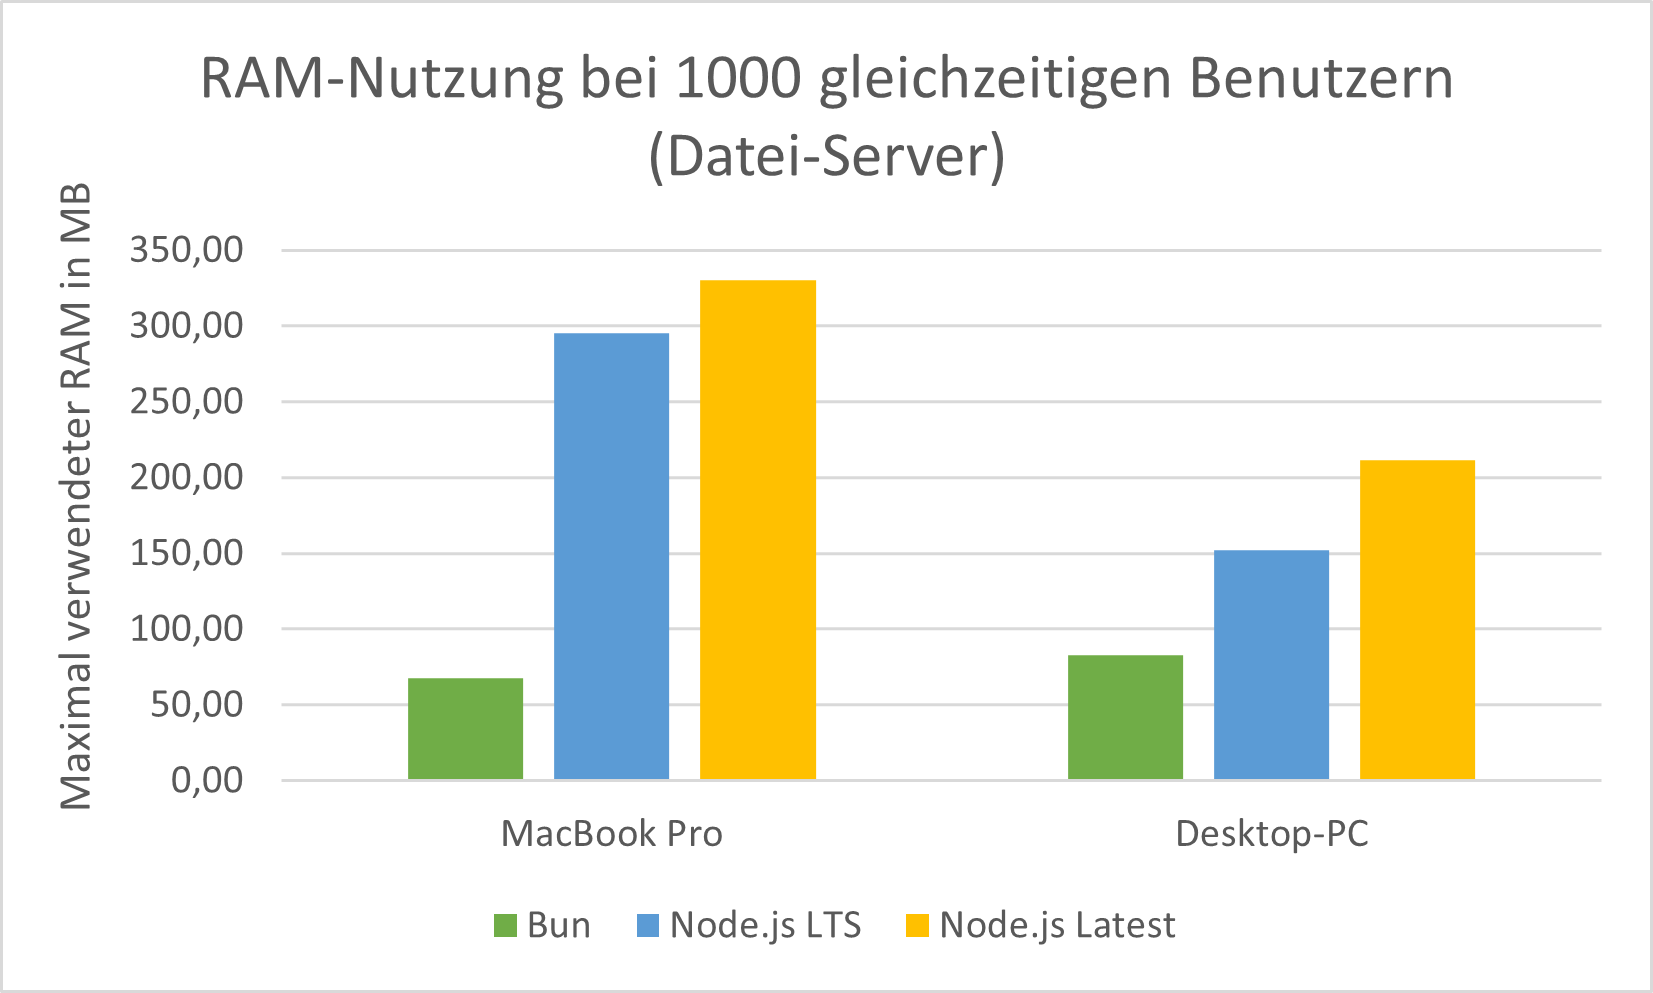
\includegraphics[width=\linewidth]{./images/fileServerRamUsage.png}
	\caption{File-Server - Maximal verwendeter Arbeitsspeicher}
	\label{fig:fileServerRamUsage}
\end{figure}


\noindent
Bei der höchsten Last werden die RAM- und CPU-Nutzung der Laufzeitumgebungen verglichen. Denn bei der höchsten Last sind die Differenzen am besten zu erkennen sein. Abbildung \ref{fig:fileServerRamUsage} zeigt den maximal verwendeten Arbeitsspeicher während des Testzeitraums von 30 Sekunden. Hier manifestiert sich der Eindruck der zuvor betrachteten Eigenschaften. Bun performt deutlich besser als Node.js, unabhängig von der verwendeten Version. Auf dem MacBook Pro benötigt Bun ca. 56 MB Arbeitsspeicher, Node.js dagegen ca. 296 MB (LTS) bzw. ca. 330 MB (Latest). Die Differenz in der RAM-Nutzung ist auf dem Desktop-PC nicht so groß wie auf dem MacBook Pro. Bun verwendete ca. 84 MB. Node.js benötigt ca. 152 MB (LTS) bzw. ca. 212 MB (Latest). Die maximale Nutzung des Arbeitsspeicher ist ein kritischer Indikator für die Effizienz bei der Speichernutzung. D. h. Bun ist hier siginfikant effizienter als Node.js. Die hohe Effizienz könnte ein Grund für die bessere Performance sein. Der Sachverhalt zeigt, dass Zig und die JavaScriptCore Engine in Bun helfen die Speichereffizienz zu steigern. Die Beobachtungen deuten auf Vorteile in der Skalierbarkeit und Kosteneffizienz hin.\\

\begin{figure}[h]
	\centering
	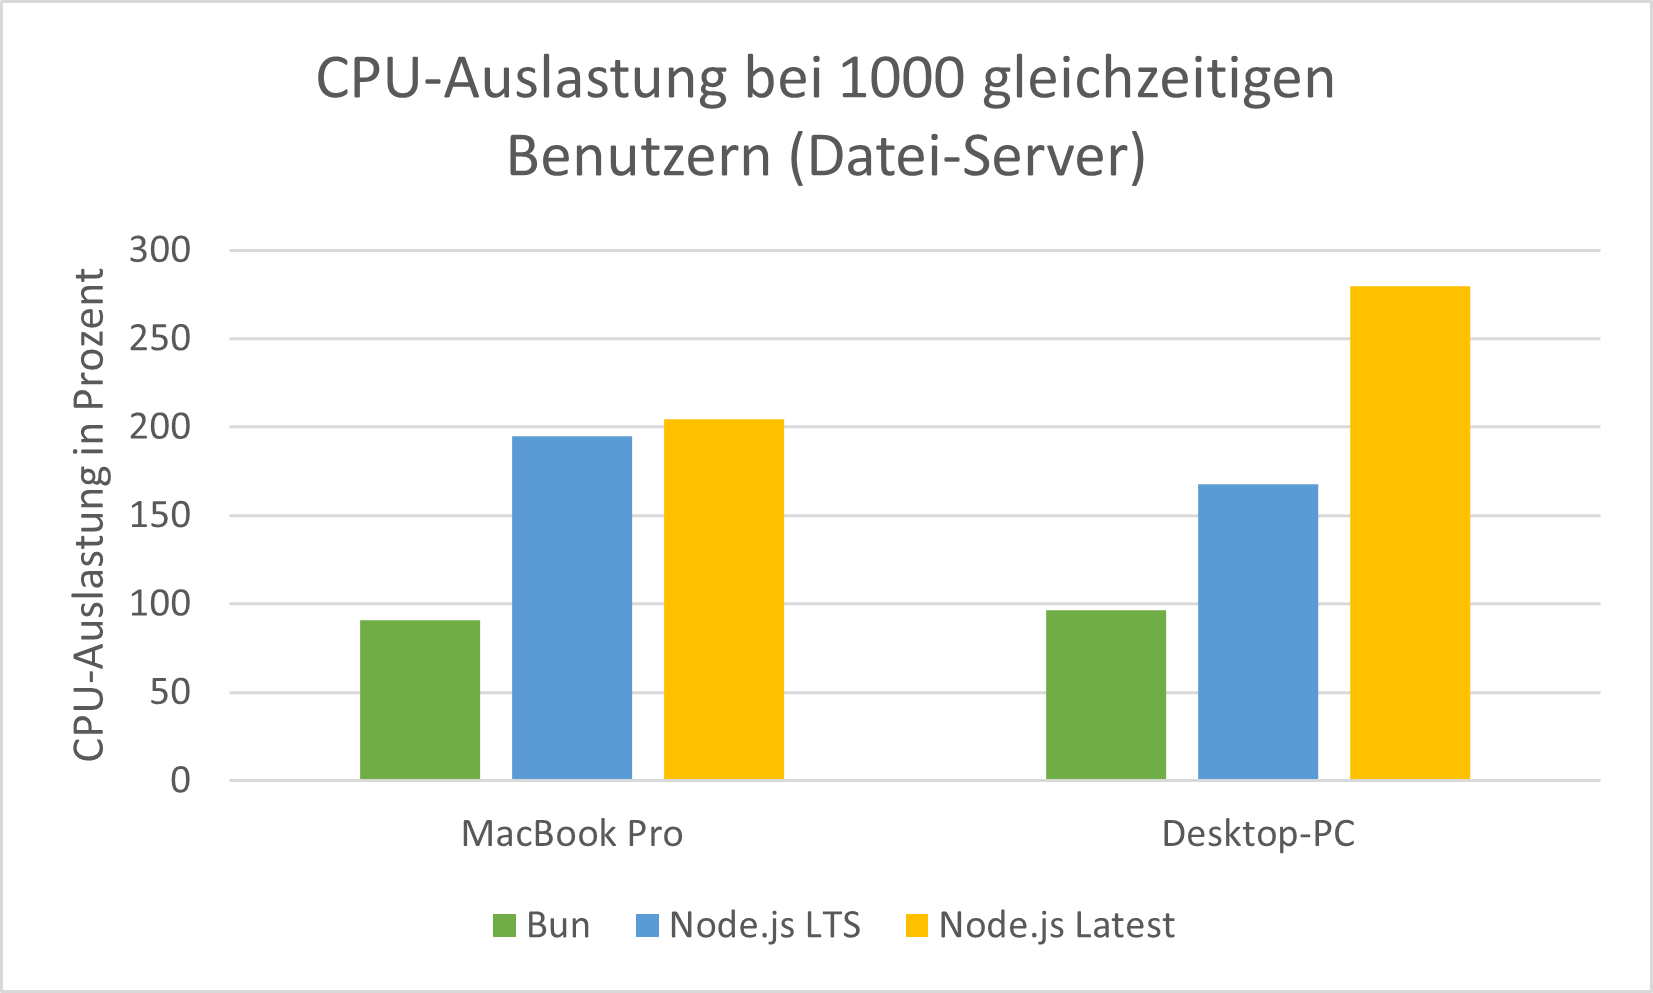
\includegraphics[width=\linewidth]{./images/fileServerCpuUsage.png}
	\caption{File-Server - CPU-Auslastung }
	\label{fig:fileServerCpuUsage}
\end{figure}

\noindent
Abbildung \ref{fig:fileServerCpuUsage} zeigt die CPU-Auslastung bei 1000 gleichzeitigen Benutzern in Prozent. \todo{Mehr als 100\% CPU Nutzung erklären} Node.js ist auch im Bereich der CPU-Nutzung weniger effizienter als Bun. Bun beansprucht ungefähr 91\% der CPU auf dem MacBook Pro und 96\% der CPU auf dem Desktop-PC. Node.js LTS benötigt ca. 195\% auf dem MacBoook Pro und 167\% auf dem Desktop-PC. Die aktuellste Version von Node.js schneidet nochmals schlechter ab. Auf dem MacBook Pro ist der Unterschied zu Node.js LTS mit einer höheren CPU-Auslastung von 10\% relativ gering. Auf dem Desktop-PC nutzt die neuste Version von Node.js 280\% der CPU im Vergleich zu 167\% bei der LTS-Version. Dies zeigt wie die Nutzung des Arbeitsspeichers, dass Bun mit den vorhandenen Ressourcen effizienter umgeht. Daraus folgt, dass Bun bei begrenzten Ressourcen intensivere Aufgaben erledigen kann.\\

\begin{figure}[h]
	\centering
	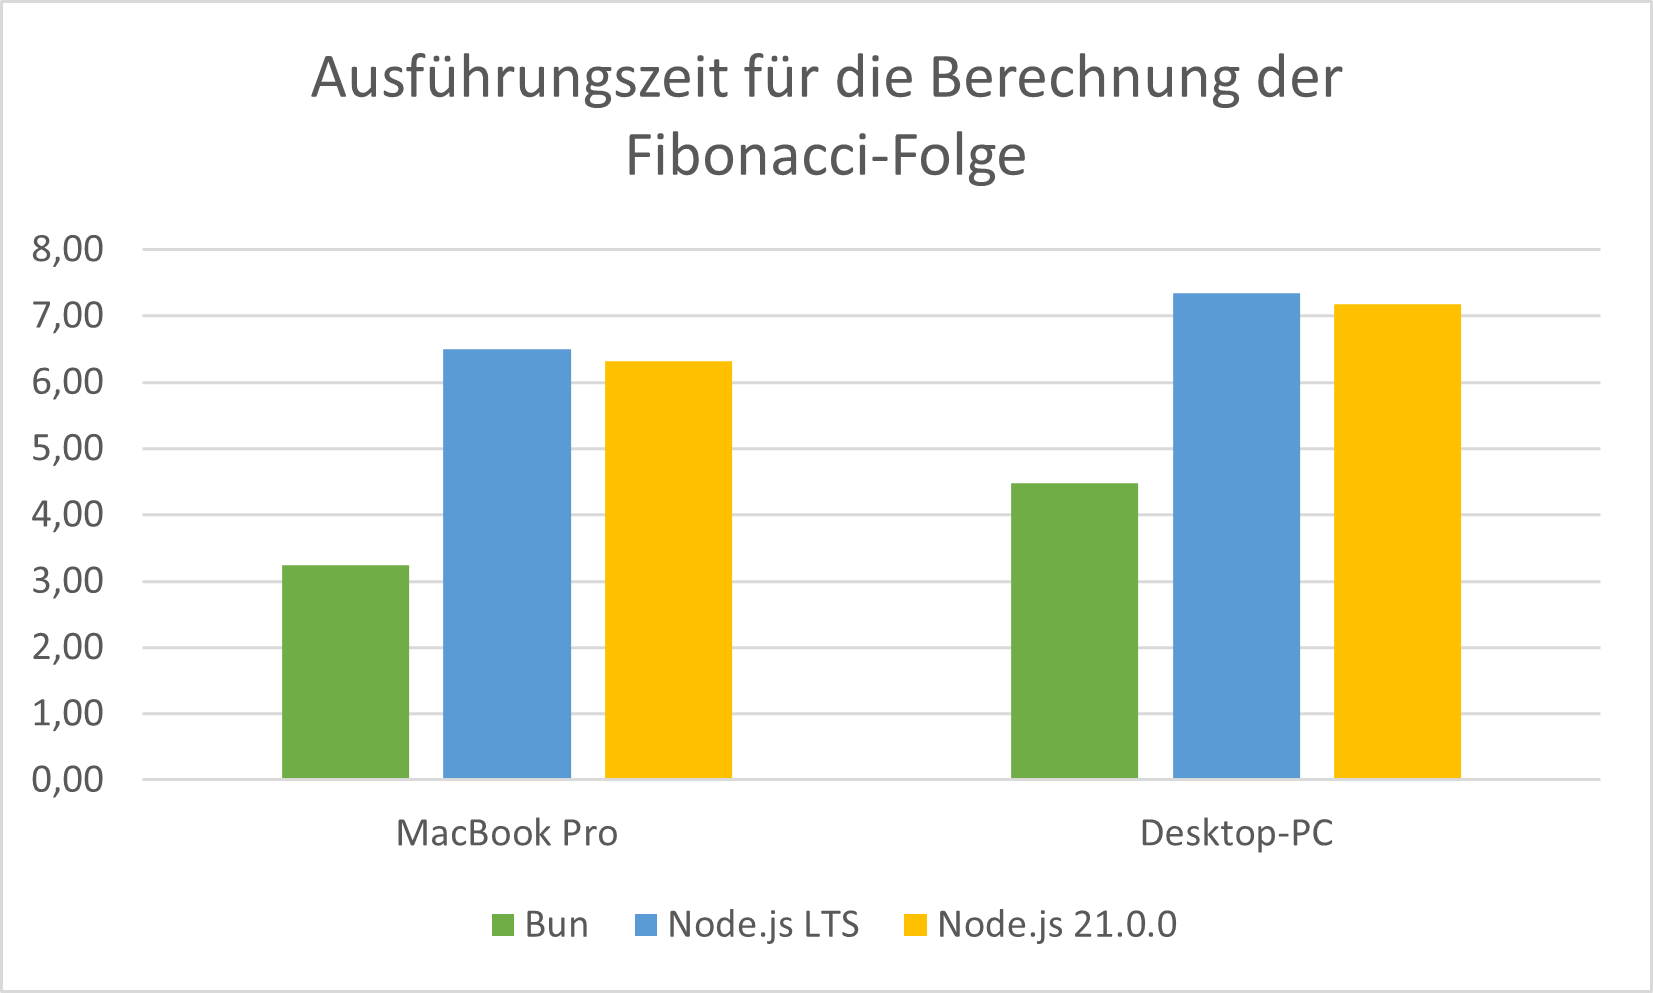
\includegraphics[width=\linewidth]{./images/fibonacciRuntime.png}
	\caption{Ausführungszeit für die Berechnung der Fibonacci-Folge}
	\label{fig:fibonacciRuntime}
\end{figure}


\noindent
Der dritte Testfall vergleicht die Leistung von Bun und Node.js bei der Ausübung rechenintensiver Aufgaben. Abbildung \ref{fig:fibonacciRuntime} veranschaulicht die benötigte Zeit für die Berechnung. Beim Berechnen der Fibonacci-Folge für die Zahl 45 benötigt Bun im Durchschnitt nur 3,24 Sekunden auf dem MacBook Pro und 4,47 Sekunden auf dem Desktop-PC. Die Versionen von Node.js unterscheiden sich kaum voneinander. Die neuste Version ist auf beiden Endgeräten ca. 0,2 Sekunden schneller als die LTS-Version. Dennoch beläuft sich die schnellste Berechnung mit Node.js auf 6,32 Sekunden auf dem MacBook Pro und auf 7,18 Sekunden auf dem Desktop-PC. Somit ist Bun auf dem MacBook Pro ca. 50\% und auf dem Desktop-PC ungefähr 40\% schneller. Die CPU-Auslastung beträgt sowohl bei Bun als auch bei Node.js ca. 100\%. Der maximal verwendete Arbeitsspeicher unterscheidet sich auf dem Desktop-PC nur um maximal 3 MB. Erwähnenswert ist, dass hier die neuste Version von Node.js 1 MB weniger Arbeitsspeicher als Bun genutzt hat. Auf dem MacBook Pro sind die Unterschiede deutlich größer. Bun benötigt maixmal ca. 26 MB RAM, Node.js im Vergleich dazu 42 MB (LTS) und 37 MB (Latest).\newline
Die Betrachtung der CPU-Auslastung, der RAM-Nutzung und der Ausführungszeiten im Kontext der Fibonacci-Folge bestätigt das Verhalten aus den zwei vorangegangenen Testszenarien. Bun besitzt eine deutlich höhere Leistung auf den genannten Endgeräten unabhängig von der betrachteten Metrik.

\section{Fazit} \label{sec:performance-conclusion}
Dieses Kapitel widmet sich auf die Beantwortung der ersten Leitfrage ``Welche konkreten Leistungsverbesserungen können in Bun 1.0 im Vergleich zu Node.js festgestellt werden, und wie lassen sie sich quantifizieren?'' (siehe Kapitel \ref{introduction}). Die Ergebnisse des Benchmarks verdeutlichen, dass Bun in sämtlichen Testszenarien signifikant bessere Leistungen als Node.js erzielt hat. Dies zeigt sich in einer deutlich reduzierten Latenz, in einer geringeren Inanspruchnahme von Arbeitsspeicher und CPU-Ressourcen während der Verarbeitung von Netzwerkanfragen. Diese Resultate bestätigen sich bei der Ausführung rechenintensiver Aufgaben. Bun hat die Fibonacci-Folge bis zu 50\% schneller berechnet als Node.js. In diesem Szenario beansprucht Bun ähnlich viel Arbeitsspeicher wie Node.js, weist jedoch eine geringere CPU-Auslastung auf. \newline
Diese Ergebnisse unterstreichen, dass Bun bei der Entwicklung gute Entscheidungen bei der Auswahl seiner Komponenten getroffen hat. Die JavaScriptCore Engine mit mehreren JIT-Kompilern (siehe Kapitel \ref{sec:foundations-Bun}) ermöglicht eine effizientere Optimierung es den Maschinencode. Die Auswahl von Zig als systemnahe Programmiersprache und das intensive Testen während der Entwicklung haben die Effizienz von Bun im Umgang mit den verfügbaren Ressourcen gesteigert. Allerdings ist die Performance nicht der alleinige Faktor bei der Wahl einer Laufzeitumgebung. Stabilität, Sicherheit, Zuverlässigkeit und auch Kompatibilität spielen eine ebenso wichtige Rolle.\\

\noindent
Das Benchmark basiert auf den Vergleich ausgewählter Eigenschaften auf einem spezifischen Hardware-Setup. Es ist zu beachten, dass diese Ergebnisse unter Verwendung von Servern aus der Produktionsumgebung potenziell abweichen können. Des Weiteren sollten weitere Eigenschaften analysiert werden, um die Überlegenheit von Bun zu verifizieren. Selbst bei einer Reproduktion des Benchmarks auf identischer Hardware kann es aufgrund unterschiedlicher Systemkonfigurationen und laufender Hintergrundprozesse zu Abweichungen kommen. \newline
Zudem beschränken sich die bisherigen Analysen auf einfache Beispiele, die sich auf die Performance der Laufzeitumgebungen konzentrieren. In der Realität sind Anwendungsquellcodes oft umfangreicher und komplexer. Die vorliegenden Ergebnisse geben daher nicht zwangsläufig die Performance solcher komplexeren Anwendungen wieder.\\

\noindent
Für eine umfassende Bewertung der Laufzeitleistung sollten die Unterschiede zwischen dem MacBook Pro und dem Desktop-PC genauer analysiert werden. Es ist wichtig, die Gründe für die signifikanten Unterschiede im Anteil erfolgreicher Anfragen zu ermitteln. Zudem sollte untersucht werden, warum die RAM-Nutzung bei der Berechnung der Fibonacci-Folge unter Ubuntu kaum variiert. Die Untersuchung sollte auf andere Hardware-Setups ausgeweitet werden, um die Generalisierbarkeit der Ergebnisse sicherzustellen.  Schließlich könnten umfangreichere Anwendungsbeispiele und realistischere Szenarien in die Analyse einbezogen werden, um die tatsächliche Performance in komplexen Umgebungen besser abzubilden.